\section{Week 2: SAT and DPLL}

\subsection{SAT}
\textbf{The satisfiability problem for propositional logic (SAT)}:
\begin{itemize}
    \item[--] \textbf{Input}: a propositional logic formula $\varphi$ (in CNF)
    \item[--] \textbf{Output}: is there a truth assignment $\alpha$ that satisfies $\varphi$?
\end{itemize}

\textbf{Reminder} solving SAT allows us to perform various reasoning tasks:
\begin{itemize}
    \item[--] $\varphi_1$ \textcolor{PineGreen}{logically entails} $\varphi_2$ ($\varphi_1 \models \varphi_2$) \\ iff $\varphi_1 \wedge \neg \varphi_2$ is \textbf{not satisfiable}.
    \item[--] $\varphi_1$ and $\varphi_2$ are \textcolor{PineGreen}{logically equivalent} ($\varphi_1 \equiv \varphi_2$) \\ iff $(\varphi_1 \wedge \neg \varphi_2) \vee (\varphi_2 \wedge \neg \varphi_1)$ is \textbf{not satisfiable}.
    \item[--] $\varphi$ is \textcolor{PineGreen}{valid} \\ iff $\neg \varphi$ is \textbf{not satisfiable}.
\end{itemize}

\textbf{Algorithms for SAT}:
\begin{itemize}
    \item Most naive algorithm: iterate over all $2^n$ truth assignments\\
    ($n$ is number of propositional variables in formula $\varphi$)
    \item All algorithms for SAT take \textbf{exponential time} in the \textbf{worst case}, but perform \textcolor{PineGreen}{very well} in practice.
    \item Most algorithms work only for \textcolor{blue}{propositional logic} formulas in \textcolor{blue}{CNF}, but translation to CNF often leads to \textbf{\textcolor{red}{exponential blow-up}} in the formula.
\end{itemize}

That's where the \textbf{\textcolor{Maroon}{Tseytin transformation}} comes in handy.

\subsection{Tseytin Transformation}
\begin{itemize}
    \item[--] We can translate an arbitrary propositional logic formula $\varphi$ efficiently to a \\ \textbf{\textcolor{WildStrawberry}{equisatisfiable CNF}} formula $\chi \text{-so } \varphi$ and $\chi$ do not have to be logically equivalent
    \begin{itemize}
        \item[$\circ$] \textbf{\textcolor{WildStrawberry}{Equisatisfiable}}: $\varphi$ is satisfiable iff $\chi$ is satisfiable. 
    \end{itemize}
    \newpage
    \item[--] The \textbf{Tseytin transformation}:
    \begin{itemize}
        \item[$\circ$] Take a formula $\varphi$ and call its variables $p_1, \cdots, p_n$.
        \item[$\circ$] Take all the subformulas $\psi_1, \cdots, \psi_m$ of $\varphi$, where $\psi_1 = \varphi$.
        \item[$\circ$] Introduce new propositional variables $q_1, \cdots, q_m$ -each $q_i$ will represent whether the subformula $\psi_i$ is satisfied.
        \item[$\circ$] For each subformula $\psi_i$, add some clauses to $\chi$:
        \begin{itemize}
            \item If $\psi_i = p_j$, \;\;\;\;\;\;\;\;\;\;\;\;\;\;\; add $(\neg q_i \vee p_j)$ and $(\neg p_j \vee q_i)$; \\
            "$(q_i \leftrightarrow p_j)$"
            \\
            \item If $\psi_i = \neg \psi_j$, \;\;\;\;\;\;\;\;\;\;\;\; add $(\neg q_i \vee \neg q_j)$ and $(q_j \vee q_i)$;  \\ "$(q_i \leftrightarrow \neg q_j)$"
            \\
            \item If $\psi_{i}=\left(\psi_{j} \wedge \psi_{k}\right)$, \;\;\;\; add $\left(\neg q_{i} \vee q_{j}\right),\left(\neg q_{i} \vee q_{k}\right)$, and $\left(\neg q_{j} \vee \neg q_{k} \vee q_{i}\right)$; \\
            $"(q_{i} \leftrightarrow q_{j} \wedge q_{k}))"$
            \\
            \item If $\psi_{i}=\left(\psi_{j} \vee \psi_{k}\right)$, \;\;\;\; add $\left(\neg q_{i} \vee q_{j} \vee q_{k}\right),\left(\neg q_{j} \vee q_{i}\right)$, and $\left(\neg q_{k} \vee q_{i}\right)$; \\
            $"(q_{i} \leftrightarrow (q_{j} \vee q_{k}))"$
            \\
            \item (and similarly for subformulas built using $\rightarrow, \leftrightarrow, ..$)
        \end{itemize} 
        \item[$\circ$] \textbf{Finally}, add the unit clause $(q_1)$.
        \item[$\circ$] Then, $\chi$ is satisfiable iff $\varphi$ is satisfiable. 
    \end{itemize}
\end{itemize}

\subsection{Algorithms}
\subsubsection{Backtracking search}
Main idea of \textbf{\textcolor{PineGreen}{Backtracking search}}:
\begin{itemize}
    \item Pick some truth value for a variable $x$, and try if that leads to a solution. If so, great!
    \item Else (if not), backtrack and try the other value.
\end{itemize}

\textbf{Useful notation}: $\left.\varphi\right|_{\ell}$ ('plugging in' $\ell$ into $\varphi$).
\begin{itemize}
    \item Let $\varphi$ be a CNF formula and $\ell$ a literal;
    \item To obtain $\left.\varphi\right|_{\ell}$ from $\varphi$:
    \begin{enumerate}
        \item Remove all clauses that contain $\ell$ (already satisfied);
        \item Remove $\neg \ell$ from all remaining clauses ($\neg \ell$ cannot be satisfied anymore)
    \end{enumerate}
\end{itemize}

\newpage
\begin{algorithm}
\SetAlgoNoEnd
\SetKwInOut{Input}{Input}
\SetKwInOut{Output}{Output}
\SetKwInput{kwAlgName}{BS$(\varphi, \alpha)$}
\caption{Backtracking search (BS)}\label{alg:BS}
\kwAlgName{}
\Input{a propositional CNF formula $\varphi$, \\ and a partial truth assignment $\alpha$ \textcolor{PineGreen}{\Comment*[r]{$\alpha$ is initially empty}} \vspace{0.1cm}} 
\Output{a satisfying truth assignment $\beta$ for $\varphi$ if it exists, otherwise “unsat” \vspace{0.1cm}}
\Begin{
    \If{$\varphi$ contains the empty clause}{\KwRet{"unsat"} \textcolor{PineGreen}{\Comment*[r]{empty clause means contradiction}}}
    \If{$\varphi$ has no clauses}{\KwRet{$\alpha$} \textcolor{PineGreen}{\Comment*[r]{no clauses means the formula is satisfied}} \vspace{0.25cm}}
    $\ell \gets$ a literal in $\varphi$ not assigned by $\alpha$\ \textcolor{PineGreen}{\Comment*[r]{the branching choice: which $\ell$}}
    \eIf{\textbf{BS}$(\left.\varphi\right|_{\ell}, \alpha \cup\{\ell\} = \beta)$}{\KwRet{$\beta$} \textcolor{PineGreen}{\Comment*[r]{first try $\ell$}}}{\KwRet{\textbf{BS}$(\left.\varphi\right|_{\neg \ell}, \alpha \cup\{\neg \ell\})$} \textcolor{PineGreen}{\Comment*[r]{if $\ell$ did not work, try $\neg \ell$}}}
}
\end{algorithm}

\begin{minipage}[t]{0.2\textwidth}
  \textbf{Ass:} $p_1$
  \centering\raisebox{\dimexpr \topskip-\height}{%
  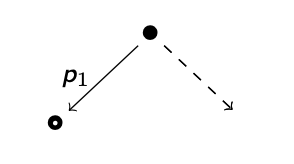
\includegraphics[width=\textwidth]{figures/bs1.png}}
  \label{fig1}
\end{minipage}
\begin{minipage}[t]{0.2\textwidth}
$$
\begin{aligned}
&\left(\text{\textcolor{red}{$\neg p_1$}} \vee \neg p_{2}\right) \\
&\left(\text{\textcolor{red}{$\neg p_1$}} \vee p_{2}\right) \\
\textcolor{Green}{\checkmark} &\left(\text{\textcolor{Green}{$p_1$}} \vee \neg p_{2}\right)
\end{aligned}
$$
\vspace{0.25cm}
\end{minipage}
\begin{minipage}[t]{0.2\textwidth}
  \textbf{Ass:} $p_1 \;\; p_2$
  \centering\raisebox{\dimexpr \topskip-\height}{%
  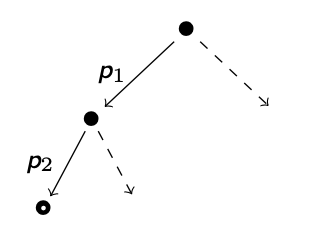
\includegraphics[width=\textwidth]{figures/bs2.png}}
  \label{fig1}
\end{minipage}
\begin{minipage}[t]{0.2\textwidth}
$$
\begin{aligned}
\text{\textcolor{red}{\xmark}} &\left(\text{\textcolor{red}{$\neg p_1$}} \vee \text{\textcolor{red}{$\neg p_{2}$}}\right) \\
\textcolor{Green}{\checkmark} &\left(\text{\textcolor{red}{$\neg p_1$}} \vee \text{\textcolor{Green}{$p_{2}$}}\right) \\
\textcolor{Green}{\checkmark} &\left(\text{\textcolor{Green}{$p_1$}} \vee \text{\textcolor{red}{$\neg p_{2}$}}\right)
\end{aligned}
$$
\end{minipage}

\begin{minipage}[t]{0.2\textwidth}
  \textbf{Ass:} $p_1 \;\; \underline{\text{$\neg p_2$}}$
  \centering\raisebox{\dimexpr \topskip-\height}{%
  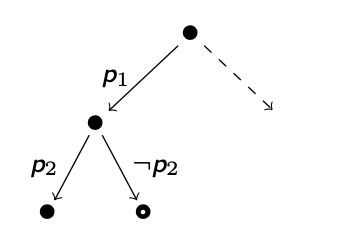
\includegraphics[width=\textwidth]{figures/bs3.png}}
  \label{fig1}
  \vspace{0.25cm}
\end{minipage}
\begin{minipage}[t]{0.2\textwidth}
$$
\begin{aligned}
\text{\textcolor{Green}{\checkmark}} &\left(\text{\textcolor{red}{$\neg p_1$}} \vee \text{\textcolor{Green}{$\neg p_{2}$}}\right) \\
\text{\textcolor{red}{\xmark}} &\left(\text{\textcolor{red}{$\neg p_1$}} \vee \text{\textcolor{red}{$p_{2}$}}\right) \\
\textcolor{Green}{\checkmark} &\left(\text{\textcolor{Green}{$p_1$}} \vee \text{\textcolor{Green}{$\neg p_{2}$}}\right)
\end{aligned}
$$
\end{minipage}
\begin{minipage}[t]{0.2\textwidth}
  \textbf{Ass:} \underline{\text{$p_1$}}
  \centering\raisebox{\dimexpr \topskip-\height}{%
  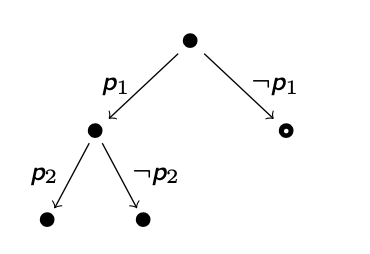
\includegraphics[width=\textwidth]{figures/bs4.png}}
  \label{fig1}
\end{minipage}
\begin{minipage}[t]{0.2\textwidth}
$$
\begin{aligned}
\text{\textcolor{Green}{\checkmark}} &\left(\text{\textcolor{Green}{$\neg p_1$}} \vee \neg p_{2}\right) \\
\textcolor{Green}{\checkmark} &\left(\text{\textcolor{Green}{$\neg p_1$}} \vee p_{2}\right) \\
&\left(\text{\textcolor{red}{$p_1$}} \vee \neg p_{2}\right)
\end{aligned}
$$
\end{minipage}

\begin{minipage}[t]{0.2\textwidth}
  \textbf{Ass:} \underline{\text{$\neg p_1$}} $p_2$
  \centering\raisebox{\dimexpr \topskip-\height}{%
  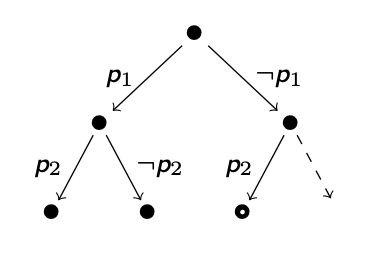
\includegraphics[width=\textwidth]{figures/bs5.png}}
  \label{fig1}
\end{minipage}
\begin{minipage}[t]{0.2\textwidth}
$$
\begin{aligned}
\text{\textcolor{Green}{\checkmark}} &\left(\text{\textcolor{Green}{$\neg p_1$}} \vee \text{\textcolor{red}{$\neg p_{2}$}}\right) \\
\textcolor{Green}{\checkmark} &\left(\text{\textcolor{Green}{$\neg p_1$}}  \vee \text{\textcolor{Green}{$p_{2}$}}\right) \\
\text{\textcolor{red}{\xmark}} &\left(\text{\textcolor{red}{$p_1$}} \vee  \text{\textcolor{red}{$\neg p_{2}$}}\right)
\end{aligned}
$$
\end{minipage}
\begin{minipage}[t]{0.2\textwidth}
  \textbf{Ass:} \underline{\text{$\neg p_1 \neg p_2$}}
  \centering\raisebox{\dimexpr \topskip-\height}{%
  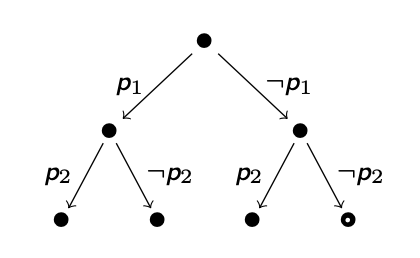
\includegraphics[width=\textwidth]{figures/bs6.png}}
  \label{fig1}
\end{minipage}
\begin{minipage}[t]{0.2\textwidth}
$$
\begin{aligned}
\text{\textcolor{Green}{\checkmark}} &\left(\text{\textcolor{Green}{$\neg p_1$}} \vee \text{\textcolor{Green}{$\neg p_{2}$}}\right) \\
\textcolor{Green}{\checkmark} &\left(\text{\textcolor{Green}{$\neg p_1$}}  \vee \text{\textcolor{red}{$p_{2}$}}\right) \\
\text{\textcolor{Green}{\checkmark}} &\left(\text{\textcolor{red}{$p_1$}} \vee \text{\textcolor{Green}{$\neg p_{2}$}}\right)
\end{aligned}
$$
\vspace{0.1cm}
\end{minipage}

In the example above, we have no empty or no clauses. We start with true, then false and go in ascending order (order picking). Furthermore the dashed line means that we still have to expand this branche later maybe. The colors indicate whether the assignment matches the literal(s). In case the color is \textcolor{red}{red}, the literal is removed from the clause. If all the literals are removed and we have a \textcolor{red}{\xmark}, that branch does not give us a solution, so we need to backtrack to the last point. A \textcolor{Green}{\checkmark} means that the clause is removed. The underlining in the assignment, means that we have no other choice anymore for that literal(s). Once all the clauses have a \textcolor{Green}{\checkmark}, we have a solution.

\newpage
\subsubsection{Propagation: unit propagation (UP)}
\textbf{Propagation}: simplifying the formula at each node in the search tree. \\
\textbf{\textcolor{Maroon}{Unit Propagation}} is a particular propagation method:
\begin{itemize}
    \item If $\varphi$ contains a \textcolor{NavyBlue}{unit clause} ($\ell$), then set the literal $\ell$ to true. 
    \item Repeat this until there are no more unit clauses (or until the formula contains the empty clause)
\end{itemize}
\vspace{0.25cm}
\textbf{\textcolor{WildStrawberry}{DPLL}} makes use of unit propagation.

\begin{algorithm}
\SetAlgoNoEnd
\SetKwInOut{Input}{Input}
\SetKwInOut{Output}{Output}
\SetKwInput{kwAlgName}{DPLL$(\varphi, \alpha)$}
\SetKwInput{kwAlgNameTwo}{UP$(\varphi, \alpha)$}
\caption{DPLL}\label{alg:BS}
\kwAlgName{}
\Input{a propositional CNF formula $\varphi$, \\ and a partial truth assignment $\alpha$ \vspace{0.1cm}} 
\Output{a satisfying truth assignment $\beta$ for $\varphi$ if it exists, otherwise “unsat” \vspace{0.1cm}}
\Begin{
    $(\varphi, \alpha) \gets \text{\textbf{UP}}(\varphi, \alpha)$ \textcolor{PineGreen}{\Comment*[r]{update $(\varphi, \alpha)$ with unit propagation}} 
    \If{$\varphi$ contains the empty clause}{\KwRet{"unsat"}}
    \If{$\varphi$ has no clauses}{\KwRet{$\alpha$} \vspace{0.25cm}}
    $\ell \gets$ a literal in $\varphi$ not assigned by $\alpha$\
    \eIf{\textbf{BS}$(\left.\varphi\right|_{\ell}, \alpha \cup\{\ell\} = \beta)$}{\KwRet{$\beta$}}{\KwRet{\textbf{BS}$(\left.\varphi\right|_{\neg \ell}, \alpha \cup\{\neg \ell\})$}}
}
\vspace{0.5cm}
\kwAlgNameTwo{}
\Begin{
    \While{$\varphi$ contains no empty clause but some unit clause $\ell$
    }{
    $\varphi \gets \left.\varphi\right|_{\ell}$ \textcolor{PineGreen}{\Comment*[r]{$\ell$ must be true, so 'plug in' $\ell$ into $\varphi$}} 
    $\alpha \gets \alpha \cup \left\{ \ell \right\}$ \textcolor{PineGreen}{\Comment*[r]{and add $\ell$ to $\alpha$}}
    }
    \KwRet{ $(\varphi, \alpha)$}
}
\end{algorithm}

The algorithm will still do some things \textcolor{red}{over} and \textcolor{red}{over again}.\\
A way to \textbf{deal} with this: \textbf{\textcolor{NavyBlue}{conflict analysis}} and \textbf{\textcolor{NavyBlue}{clause learning}}.

\newpage
\subsubsection{Conflict graph (implication graph)}

Example of a \textbf{conflict graph}:
\begin{figure}[ht!]
% 	\centering
	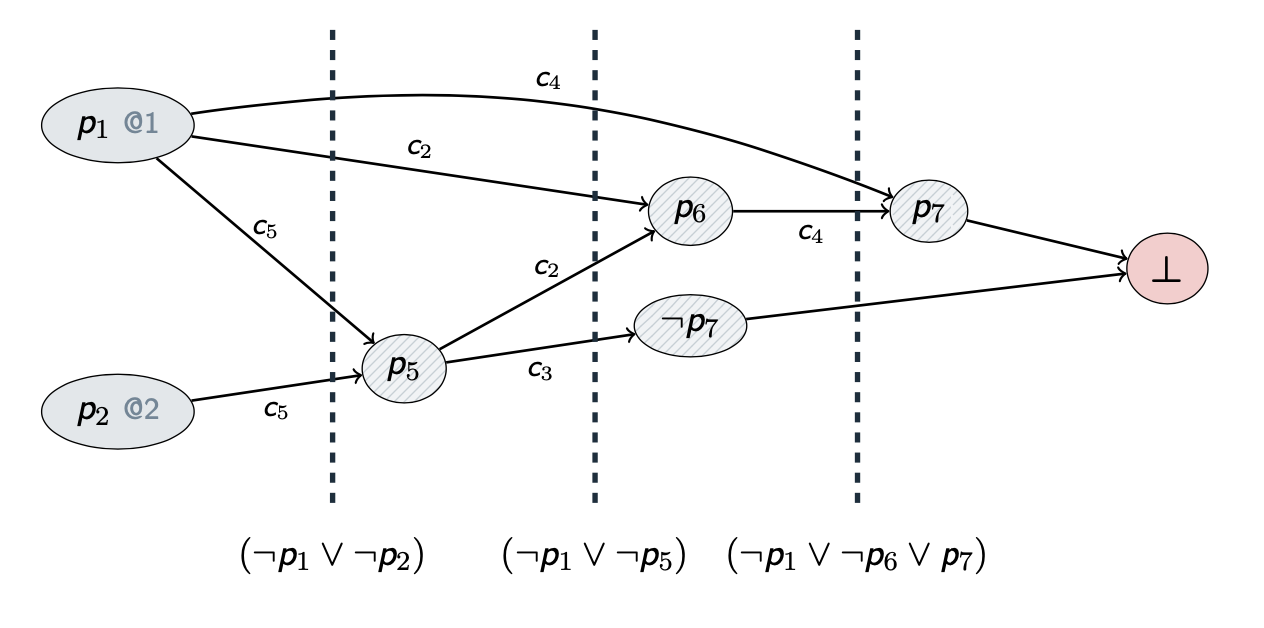
\includegraphics[height=5cm]{figures/conflict graph.png}
	\label{fig:conflict}
\end{figure}

The \textbf{\textcolor{NavyBlue}{implication graph}} is a directed graph that is constructed as follows:
\begin{itemize}
    \item Add a node for each decision literal—i.e., literals that can still be backtracked on.
    \item Every time unit propagation has been used with some clause $(\ell_1 \vee \cdots \vee \ell_k)$ to conclude, say, $\ell_k$ draw an edge from the nodes for $\neg \ell_1, \cdots, \neg \ell_{k-1}$ to the node for $\ell_k$ (and label these edges with the clause number).
    \item Add a node for the conflict (with label $\perp$), and for any two nodes for negated literals (i.e., $\ell$ and $\neg \ell$), draw an edge from these nodes to the conflict node.
\end{itemize}

For each state of the algorithm, there is a unique implication graph—that might contain several pairs of conflicting literals.
\\
\\
A \textbf{\textcolor{Maroon}{conflict graph}} is a subgraph of the \textcolor{NavyBlue}{implication graph} that contains exactly one conflicting pair of literals:
\begin{itemize}
    \item Pick some conflicting pair $\ell, \neg \ell$ of literals in the implication graph, together with the conflict node $\perp$.
    \item Keep only those nodes that have a path to either $\ell$ or $\neg \ell$, and remove all other nodes from the implication graph.
\end{itemize}

\subsubsection{Further additions to DPLL}
\begin{itemize}
    \item \textbf{Pure literal elimination (PL)}: if $\varphi$ contains a literal $\ell$ but not $\neg \ell$, then you can safely set $\ell$ to true.
    \item \textbf{Backjumping}: learning a clause can enable backtracking several choices at once
    \item \textbf{Branching heuristics}: pick a literal $\ell$ that immediately satisfies as many clauses as possible
    \item \textbf{Random restarts}: Restart search every now and then (keep learned clauses).
\end{itemize}

\subsection{SAT and NP-completeness}
A problem Q is \textbf{\textcolor{NavyBlue}{NP-complete}} if every other problem Q' in the class NP can be efficiently (in polynomial-time) be reduced to it (and if Q is in NP).
\begin{itemize}
    \item A \textcolor{red}{reduction} is an algorithm $p$ that maps an input $x^\prime$ for $Q^\prime$ to an input $x$ for $Q$ such that the outputs are the same—e.g., $Q(x) = Q^\prime(x^\prime)$.
\end{itemize}

\textbf{SAT} is \textbf{\textcolor{NavyBlue}{NP-complete}}.

\newpage